\documentclass[tikz]{standalone}
\usepackage[utf8]{inputenc}

\usepackage{modml}

\tikzset{%
  highlight/.style={rectangle,rounded corners,fill=green!15,draw,fill opacity=0.5,inner sep=0pt}
}
\newcommand{\tikzmark}[2]{\tikz[overlay,remember picture,baseline=(#1.base)] \node (#1) {#2};}
%
\newcommand{\HighlightColumn}[1]{%
    \tikz[overlay,remember picture]{
    \node[highlight,fit=(top#1.north west) (bottom#1.south east)] (column#1) {};}
}

\newcommand{\HighlightRow}[1]{%
    \tikz[overlay,remember picture]{
    \node[highlight,fit=(left#1.north west) (right#1.south east)] (row#1) {};}
}

\newcommand\sol[1]{\tikz[overlay, remember picture,baseline=-\the\dimexpr\fontdimen22\textfont2\relax]\node[rectangle,fill=blue!50,rounded corners,fill opacity = 0.2,text opacity =1] {$#1$};} 


\begin{document}
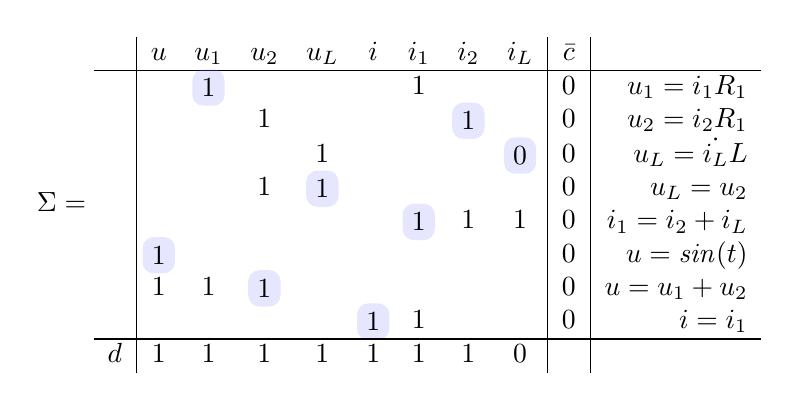
\begin{tikzpicture}
\node(matrix) {
$
  \Sigma = \begin{array}{l|cccccccc|c|r}      
    & u & u_1 & u_2 & u_L & i & i_1 & i_2 & i_L & \bar{c} & \\
    \hline
    
    &  & \sol{1} &  &  &  & 1 &  &  & 0 & u_1 = i_1R_1 \\
    
    &  &  & 1 &  &  &  & \sol{1} &  & 0 & u_2 = i_2R_1 \\
    
    &  &  &  & 1 &  &  &  & \sol{0} & 0 & u_L = \dot{i_L}L \\
    
    &  &  & 1 & \sol{1} &  &  &  &  & 0 & u_L = u_2 \\
    
    &  &  &  &  &  & \sol{1} & 1 & 1 & 0 & i_1 = i_2 + i_L \\
        
    & \sol{1} &  &  &  &  &  &  &  & 0 & u = \mathit{sin}(t) \\
    
    & 1 & 1 & \sol{1} &  &  &  &  &  & 0 & u = u_1 + u_2 \\
    & \tikzmark{left3}{$$} &  &  &  & \sol{1} & 1 &  &  & \tikzmark{right3}{$0$} & i = i_1 \\
    \hline    
    \bar{d} & 1 & 1 & 1 & 1 & 1 & 1 & 1 & 0 & 
    \end{array}
$
};
\end{tikzpicture}
\end{document}​
